\RequirePackage[l2tabu, orthodox]{nag}
\documentclass{report}

\usepackage{hyperref}
\usepackage{graphicx}

\graphicspath{{figure/}{fig/}{logo/}{logos/}{graph/}{graphs}}
\DeclareGraphicsExtensions{.pdf,.eps,.png,.jpg,.jpeg}

\makeatletter
\newcommand*{\rom}[1]{\expandafter\@slowromancap\romannumeral #1@}
\makeatother

\title{\textbf{Notes on CDE\footnote{\url{http://www.pgbovine.net/cde.html}}}}
\author{Hongxu Chen}
\date{2014-01-04}

\begin{document}
\maketitle

\textbf{CDE} uses system call interposition(\textsl{\textbf{ptrace}}, \textsl{\textbf{strace}}) to
monitor the execution of x86-Linux programs and \emph{automatically} package up
the \textbf{C}ode, \textbf{D}ata, and \textbf{E}nvironment required to run them
on other x86-Linux machines, requiring no \textmd{installation},
\textmd{configuration}, or \textmd{root permissions}, thereby eliminating
\textsl{dependency hell}

\section{Problems for Software Packages}
The path from having a piece of software running on the own machine (\rom{1}) to
getting it running on machine (\rom{2}) is fraught with potential pitfalls.\\
\begin{itemize}
\item The programmer might:
  \begin{itemize}
  \item Forget to document \textsl{a crucial step} needed during installation
  \item Forget to list a \textsl{library version} dependency, leading to run-time errors when the wrong version gets silently run on the user’s machine
  \item List the right library version, but one which is either \textsl{hard to obtain} or \textsl{conflicts} with a library needed by a different program on the user’s machine
  \end{itemize}
\item The software itself might require libraries depending on many other libraries, which themselves need to be transitively obtained and installed by the user, leading to an aggravating experience known as \textsl{dependency hell}
\item The user might lack the \textsl{permissions} or \textsl{willingness} to risk installing software packages as root in the first place
\end{itemize}

\section{Workflow of CDE}

\subsection{Procedures}
\label{sec:procedures}

The whole documentation can be seen at {\url{http://www.pgbovine.net/cde/manual/index.html#quick-start}}
\begin{itemize}
\item \textsf{Prepend} any Linux command with the \textbf{cde} executable. cde executes your command and uses \emph{ptrace} system call interposition to collect \textbf{code}, \textbf{data files}, and \textbf{environment} variables used during execution into a \emph{self-contained} package.
\item \textsf{Copy} the resulting package to any modern x86 Linux machine.
\item Change into the package directory and prepend the original command with the \textbf{cde-exec} executable. \textsf{cde-exec} loads the stored environment variables and then uses ptrace to redirect file-related system calls so that executables and libraries can load the required dependencies from within the package.
\end{itemize}

\subsection{An Example}
\label{sec:an-example}
\begin{figure}[t]
  \centering
  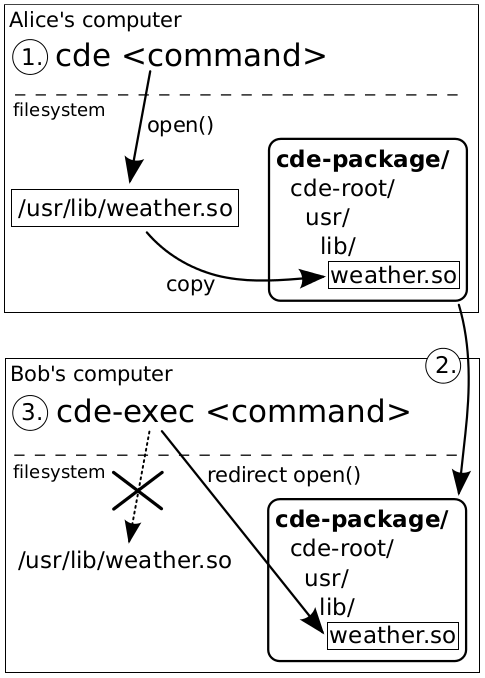
\includegraphics[width=.8\textwidth]{CDE_example.png}
  \caption{Example Use of CDE}
\end{figure}

\begin{enumerate}
\item Run the following At x86-Linux computer (\rom{1})
\begin{verbatim}
cde python weather_sim.py tokyo.dat
\end{verbatim}
\item A directory \textbf{cde-package} will be generated at (\rom{1}):
\begin{verbatim}
cde-package/
cde-package/cde-root
...
cde-package/cde-root/bin
cde-package/cde-root/usr/python
cde-package/cde-root/usr/lib/weather.so
...
cde-package/cde.uname
cde-package/cde.options
cde-package/cde-exec
cde-package/cat.cde
cde-package/cde.log
cde-package/cde.full-environment
\end{verbatim}
\item copy directory into another x86-Linux machine (\rom{2}), inside
  \textbf{cde-package}, run the command accordingly with \textbf{cde-exec} prepended.
\begin{verbatim}
cde-exec python weather_sim.py tokyo.dat
\end{verbatim}
\end{enumerate}

\section{Use Cases}
\begin{itemize}
\item Reproducible research: for other researchers and probably the authors
\item Distributing software
\item Running software without perturbing the OS
\item Deploying computations to a cluster
\item Demoing a prototype to clients
\item Running software on an incompatible OS version
\end{itemize}

\section{Design \& Implementation}

\subsection{Create a new package with CDE}
\begin{enumerate}
\item Primary action: use \textsl{ptrace} to monitor the target program’s system calls and \textsl{copy} all of its accessed files into a self-contained package.
\item Copying files into package
\item Mutate filesystem: e.g. rename corresponding files
\item Updating current working directory
\item Tracking sub-processes and threads
\item \textbf{execve}
\end{enumerate}

\subsection{Executing a package with cde-exec}
\begin{enumerate}
\item Primary action: use ptrace to redirect file paths that the target program
requests into the package.
\item Implementing syscall rewriting
\item Spoofing current working directory
\end{enumerate}

\section{Related Work}
\begin{enumerate}
\item Mac OS X bundles
\item VMware ThinApp(Windows): must monitor \textsf{installation}
\item Virtual Machine
\item \textsl{ptrace} tools
  \begin{itemize}
  \item secure sandboxes
  \item record-replay systems
  \item user-level filesystems
  \end{itemize}
\end{enumerate}

\section{Issues \& Improvements}

\subsection{Limitations}
Executing a command within a CDE package will fail if:
\begin{itemize}
\item the Linux kernel or hardware architecture is incompatible with the
  binaries in the package $\rightarrow$ virtualization/emulation helps
\item the arguments or input change to make the program load a new shared
  library that the original execution did not load $\rightarrow$ IMPROVEMENTS
\item the arguments or input change to make the program load another file that
  is not in the package $\rightarrow$ don't deal with it(or add related files manually)
\end{itemize}
Also Limited by the limitations of ptrace and of executing binaries by explicitly invoking the dynamic linker

\subsection{Possible Improvements(my thoughts)}
\label{sec:poss-impr}

\begin{itemize}
\item \textbf{CDE} mainly works for application programs $\rightarrow$ more
  system applications?
\item \textbf{dynamically} deployment requires additional cost $\rightarrow$
  statically or a mixture?
\item only deal with ONE path(although possibly works for a few different
  inputs) $\rightarrow$ symbolly run or fuzzy testing ?
\end{itemize}

\end{document}